\section{Pendolo}

La seconda parte di questa relazione tratta l'esperienza di misura del periodo
di un pendolo. Lo scopo dell'esperienza è imparare a trattare gli errori
casuali, dovuti alla procedura di misurazione del periodo con un cronometro,
che introduce inevitabilmente fluttuazioni casuali nelle misure effettuate,
e gli errori sistematici, dovuti alla diversa prontezza di riflessi degli
sperimentatori. In questo ultimo caso sorge il problema della 
compatibilità delle misure effettuate dai tre diversi membri del gruppo.

Ci siamo anche posti il problema di verificare sperimentalmente la
correttezza della legge del pendolo semplice, cosa che ogni studente di
fisica dovrebbe fare almeno una volta nella sua vita!

\subsection{Descrizione della procedura di misura}

\subsubsection{Apparato sperimentale}

Il pendolo è stato realizzato con un filo da pesca, che si può considerare
inestensibile, fissato con un morsetto al supporto del tavolo da laboratorio.
All'altra estremità del cavo è stato appeso, attraverso un gancio, un corpo
cilindrico di metallo di massa $m$ = 205 g. Il pendolo si può schematizzare,
trascurando il gancio, come un cavo di lunghezza $l_c = 55.8 \pm 0.2$ 
cm unito ad un cilindro omogeneo di altezza $h = 5.1 \pm 0.05$ cm.
Le incertezze riportate nelle misure sono dovute a difficoltà incontrate nella
misurazione e alla risoluzione del metro a nastro che abbiamo usato.
Non abbiamo ritenuto di poter fare meglio di così.

\subsubsection{Predizione teorica (??? spostare? ???)}

Per il calcolo teorico del periodo è stato utilizzato il modello del pendolo
semplice, che abbiamo considerato adeguato alla situazione. La massa $m_c$ del
cavo è stata considerata trascurabile, o meglio poiché $m_c \ll m$ si è posto
$m_c = 0$. Inoltre, dato che in realtà
il cilindro non è puntiforme, lo abbiamo approssimato ad un punto
materiale posizionato nel suo baricentro, che si trova ad una distanza
$\frac{h}{2}$ dal punto di sospensione del corpo.
Nel modello del pendolo semplice, la lunghezza del cavo è quindi
$l = l_c + \frac{h}{2} = (55.8 \pm 0.2 \, cm) + (2.5 \pm 0.025 \, cm) = 58.3 \pm 0.225 \, cm = 0.583 \pm 0.00225 \, m$.
Il valore di $g$, l'accelerazione di gravità, non è stato da noi misurato,
quindi abbiamo considerato $g = 9.8 \pm 0.02 \, \frac{m}{s^2}$, un
valore molto prudente. Con questi valore di $l$ e $g$ si ottene un periodo:

\begin{equation}
    \mathcal{T} = 2\pi \sqrt{\frac{l}{g}} = 1.533 \pm 0.003 \, s 
\end{equation}

Questo valore è quindi il valore atteso di periodo del pendolo. Lo scopo
dell'esperimento è quello di verificare sperimentalmente se questa predizione
è corretta.

%% da spostare più in giu??? forse sotto a "Processo di acquisizione dei dati sperimentali"?
\subsubsection{Errori sistematici (spostare???)}

Al fine di evitare errori sistematici riguardanti il modello teorico,
cioè errori causati dal fatto che il modello teorico non rispechia l'apparato
sperimentale usato, sono state prese le seguenti precauzioni:

\begin{itemize}
    \item{Si è tentato di contenere le oscillazioni del pendolo in un
        unico piano verticale. Abbiamo notato che a causa delle
        vibrazioni al momento del rilascio, il pendolo tende a seguire una
        traiettoria ellittica, invece che compiere la sua oscillazione su di un piano.
        Nei casi in cui la traiettoria si discostasse significativamente dal piano
        si è quindi proceduto a ripetere da capo la misura.}
    
    \item{Durante le operazioni di misura abbiamo mantenuto il massimo numero
        di oscillazioni entro il valore 20-30 affinché l'attrito con l'aria
        non influisse in modo significativo sul periodo del pendolo.}

    \item{Ci siamo accertati che l'ampiezza massima delle
        oscillazioni non superasse i 10$^\circ$ dalla verticale, in modo che
        l'approssimazione lineare $sin(\vartheta) \simeq \vartheta$ che viene
        utilizzata per calcolare la legge del pendolo sia accettabile. Infatti, per un
        angolo $\vartheta = 10^\circ = 0.175 \,\, rad$ si ha che:}

    \begin{equation}
        sin(\vartheta) = 0.174 \qquad \frac{\vartheta}{sin(\vartheta)} = 1.005
        \label{eq:theta_su_sintheta}
    \end{equation}

\end{itemize}

Possiamo stimare l'errore sistematico commesso. Poichè nella (\ref{eq:theta_su_sintheta})
abbiamo ottenuto un errore del 5 per mille l'errore sistematico dovuto a tutte le
cause elencate sopra è sicuramente maggiore di questo valore. Ci sentiamo abbastanza
sicuri stimando l'errore:

\begin{equation}
    \sigma_{sys} = 4 \cdot \frac{\vartheta}{sin(\vartheta)} = 2 \%
    \label{eq:errore_sistematico}
\end{equation}

% Non so se questo è effettivamente interessante ai fini della discussione:
[Tramite il disegno dell'angolo massimo su un foglio di carta appositamente
posizionato vicino al punto di sospensione del filo.]

Tra gli errori sistematici segnaliamo, inoltre, il fatto che le misure sono state
effettuate da sperimentatori diversi, che introducono degli errori sistematici
che variano da persona a persona. Questi errori saranno trattati nella sezione
di analisi dei dati, e non sono stati inclusi nella (\ref{eq:errore_sistematico}).

%% frase un po' scema???
Le precauzioni prese dovrebbero essere sufficienti a ridurre l'errore sistematico
entro limiti accettabili. Tuttavia è risaputo che gli errori sistematici
sono i più difficili da scovare ed eliminare.
	
\begin{table}[bt]
	\begin{tabular} {c c c c | c c c c | c c c c}
		\toprule
		\multicolumn{12}{c}{Periodo del pendolo [s]} \\
		\multicolumn{4}{c}{Francesco} & \multicolumn{4}{c}{Davide} & \multicolumn{4}{c}{Andrea} \\
		\midrule
		15.04 & 14.99 & 14.99 & 14.97 & 14.91 & 14.97 & 15.06 & 15.04 & 14.98 & 14.98 & 15.05 & 15.01 \\
		14.99 & 14.99 & 15.01 & 15.08 & 14.92 & 15.06 & 15.08 & 15.02 & 14.85 & 14.99 & 14.98 & 15.00 \\
		15.04 & 15.00 & 15.06 & 14.98 & 15.06 & 15.02 & 15.04 & 15.00 & 15.04 & 14.99 & 14.99 & 14.94 \\
		14.93 & 14.98 & 14.98 & 15.04 & 15.06 & 15.06 & 15.02 & 14.91 & 15.01 & 15.00 & 15.13 & 14.99 \\
		14.99 & 14.91 & 15.03 & 15.03 & 15.03 & 15.02 & 15.06 & 15.02 & 14.88 & 15.01 & 15.02 & 14.96 \\
		\bottomrule
	\end{tabular}

	\caption{Tabella delle misure del periodo del pendolo ottenute dai 3 membri del gruppo.
        Ogni sperimentatore ha raccolto 20 misure di 10 periodi. Sono riportati
        i dati grezzi di lettura del cronometro, riferiti a 10 periodi. }
    \label{tab:pendolo}
\end{table}

\subsubsection{Processo di acquisizione dei dati sperimentali}

Per le misurazioni è stato utilizzato un comune cronometro con risoluzione di
misura pari a 0.01 s. [errore di risoluzione???] Ogni componente del gruppo ha
cronomerato 20 volte il tempo impiegato dal pendolo per compiere 10 periodi.
I valori grezzi misurati, riportati nella tabella \ref{tab:pendolo}, sono stati divisi per
10 per ottenere il valore medio del periodo del pendolo. Questo ci ha permesso
di diminuire gli errori sistematici dovuti alla prontezza di riflessi dei diversi
operatori, che verranno trattati più approfonditamente della sezione di analisi dei
dati, e di aumentare la risoluzione del cronometro fino a 1 millisecondo.

Successivamente un componente del gruppo ha eseguito 100 misurazioni di periodi
singoli dell'apparato, riportate nella tabella \ref{tab:pendolo100}. L'aquisizione di dati è stata
effettuata con la seguente procedura:

% si può forse togliere l'elenco???
\begin{enumerate}
    \item{Il pendolo è stato fatto oscillare prestando attenzione al piano di oscillazione
        e all'ampiezza dell'oscillazione.}

    \item{Si è misurato un periodo, annotato il valore ottenuto e azzerato il cronometro.}

    \item{Le misurazioni sono state intervallate da 1-2 periodi non misurati.}

    \item{Ogni 10 misurazioni, che equivale a meno di 30 periodi, il pendolo è stato fermato
        e fatto ripartire, per evitare lo smorzamento dovuto all'attrito con l'aria.}
\end{enumerate}

Non è stato utilizzata la funzione «giro» del cronometro, al fine di evitare
di introdurre dipendenza tra le varie misure. Azzerando il cronometro ogni 
volta le misure risultano statisticamente indipendenti.

\begin{SCtable}[][tb]
	\centering
	\begin{tabular} {c c c c c | c c c c c}
		\toprule
		\multicolumn{10}{c}{Periodo del pendolo - Misure di un operatore [s]} \\
		\midrule
		1.46 & 1.54 & 1.55 & 1.57 & 1.41 & 1.45 & 1.52 & 1.45 & 1.37 & 1.53 \\
		1.57 & 1.50 & 1.52 & 1.50 & 1.48 & 1.49 & 1.44 & 1.49 & 1.43 & 1.53 \\
		1.50 & 1.50 & 1.56 & 1.61 & 1.45 & 1.38 & 1.52 & 1.41 & 1.60 & 1.49 \\
		1.48 & 1.53 & 1.52 & 1.55 & 1.54 & 1.46 & 1.51 & 1.51 & 1.49 & 1.52 \\
		1.52 & 1.50 & 1.48 & 1.46 & 1.41 & 1.48 & 1.45 & 1.48 & 1.52 & 1.51 \\
		\midrule
		1.55 & 1.52 & 1.55 & 1.49 & 1.51 & 1.50 & 1.52 & 1.49 & 1.54 & 1.52 \\
		1.45 & 1.49 & 1.47 & 1.47 & 1.48 & 1.48 & 1.53 & 1.51 & 1.52 & 1.47 \\
		1.54 & 1.42 & 1.43 & 1.45 & 1.49 & 1.42 & 1.47 & 1.36 & 1.50 & 1.55 \\
		1.58 & 1.52 & 1.45 & 1.48 & 1.44 & 1.52 & 1.51 & 1.50 & 1.54 & 1.52 \\
		1.52 & 1.52 & 1.47 & 1.52 & 1.44 & 1.56 & 1.50 & 1.49 & 1.52 & 1.56 \\
	\bottomrule
	\end{tabular}
	\caption{Misure di periodo effettuate da uno dei tre componenti del gruppo.
        Sono riportati i valori di lettura del cronometro riferiti a singole oscillazioni
        (periodi) dell'apparato.}
    \label{tab:pendolo100}
\end{SCtable}

\subsection{Analisi dei dati}

\subsubsection{Dati dei tre operatori}

La Tabella \ref{tab:pendolo} e la Figura \ref{fig:pendolo} riguardano i 60 dati
relativi alla misura del periodo del pendolo da parte di tutti e tre i
componenti del gruppo.

\begin{figure}[p]
	\centering
	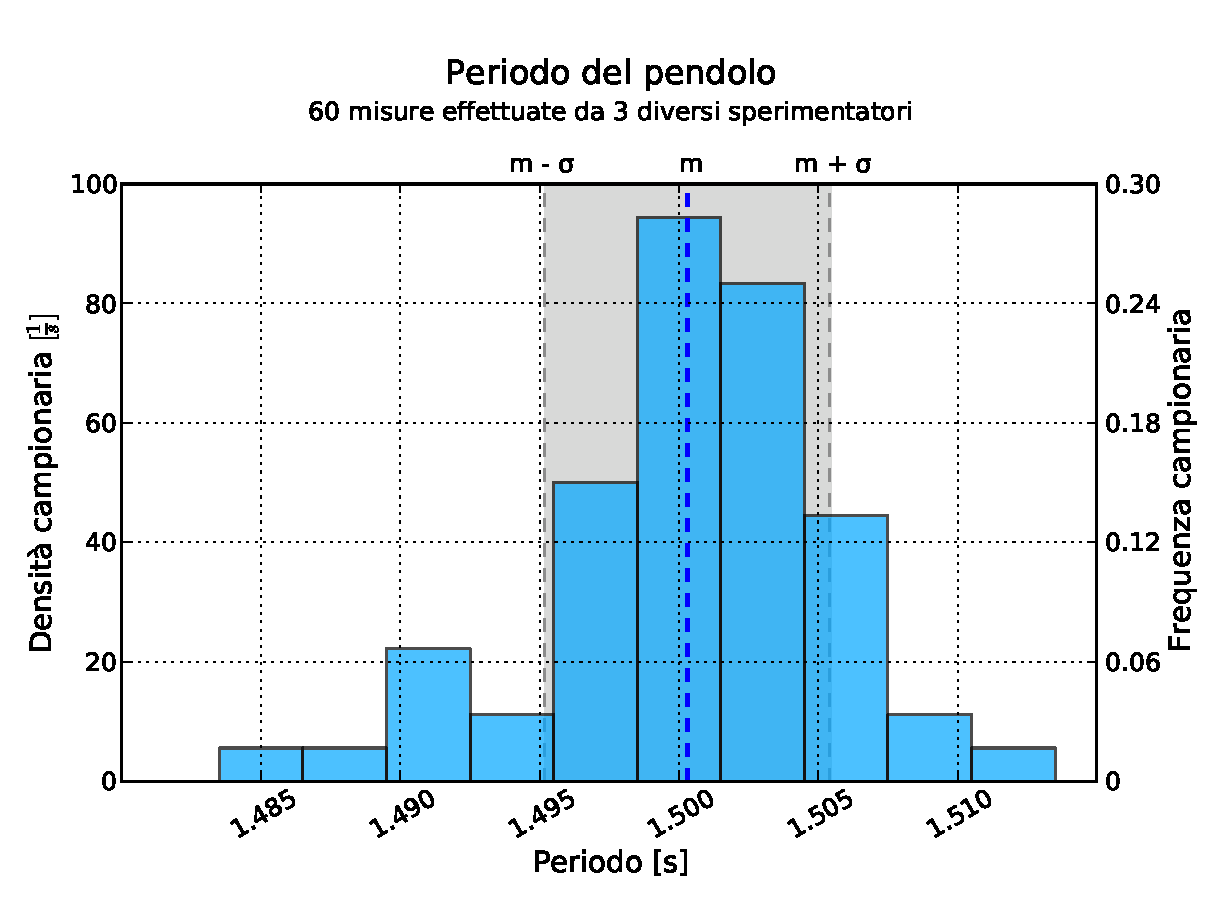
\includegraphics[width=120mm]{grafici/Pendolo.pdf}
	\caption{L'istogramma mostra le misure effettuate da tutti e tre gli sperimentatori.
        È indicato l'intervallo di incertezza tipo e la media campionaria. La larghezza
        dei bin dell'istogramma è 0.003 s. Come si può notare la forma dell'istogramma
        assomiglia ad una distribuzione gaussiana, come era prevedibile sapendo che gli
        errori dominanti delle misure sono casuali.}
    \label{fig:pendolo}
\end{figure}

\begin{figure}[p]
	\centering
	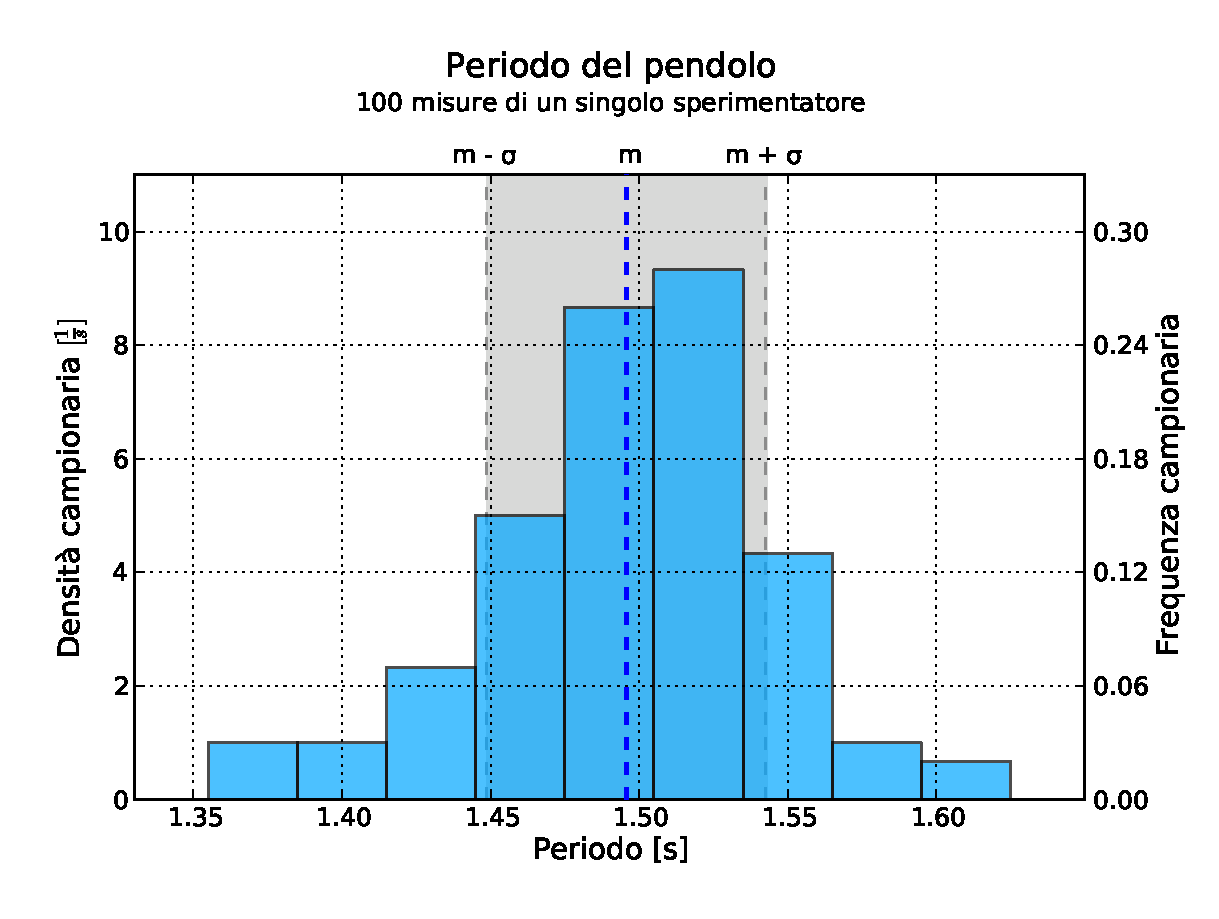
\includegraphics[width=120mm]{grafici/Pendolo100.pdf}
	\caption{Istogramma delle 100 misure di periodo del pendolo ottenute
        da un membro del gruppo. Sono evidenziate la media campionaria
        e l'intervallo di incertezza tipo. Come notato nella figura \ref{fig:pendolo}
        anche qui la distribuzione somiglia ad una distribuzione normale,
        a causa degli errori causali.}
    \label{fig:pendolo100}
\end{figure}

\begin{figure}[bt]
	\centering
	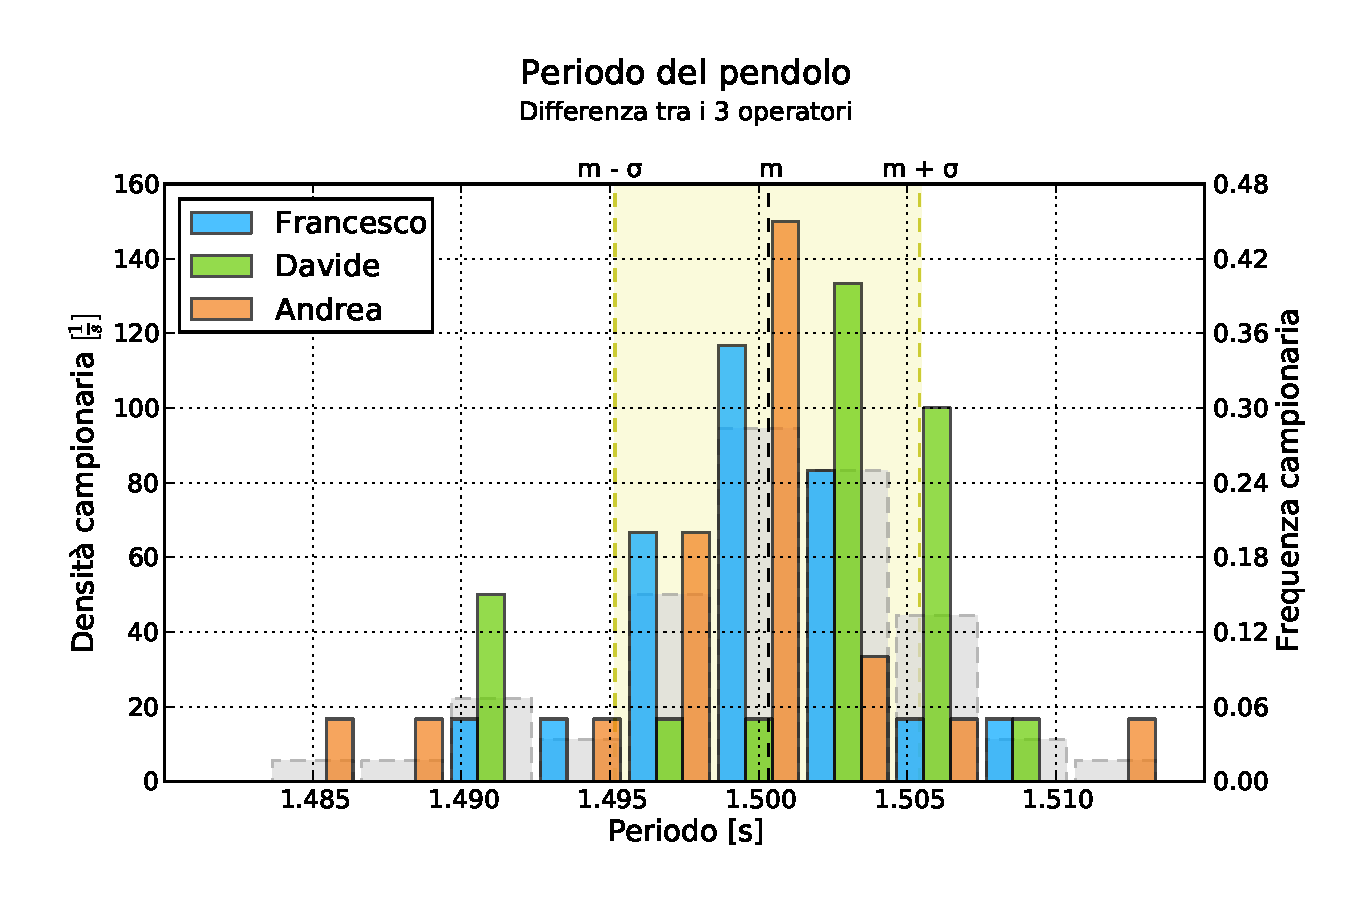
\includegraphics[width=150mm]{grafici/pendolo3.pdf}
	\caption{Il grafico illustra le misure di periodo del pendolo ottenute
        dai 3 diversi membri del gruppo, mettendo in risalto gli errori
        sistematici commessi. Da notare il fatto che Davide ha registrato più
        misure nel bin centrato in 1.503 e ha media campionaria più alta, mentre gli
        altri sperimentatori hanno picchi nel bin centrato in 1.500. In sottoimpressione
        è disegnato l'istogramma con i dati di tutti e 3 i componenti del gruppo, riportato
        anche in figura \ref{fig:pendolo}.}
    \label{fig:pendolo3}
\end{figure}

\paragraph{Compatibiltà delle misure di diversi sperimentatori.}

La prima cosa che ci proponiamo di dimostrare è la compatibiltà
tra i dati misurati da ognuno di noi. Fissiamo a priori un fattore
di copertura $k$ = 2. Date due misure $x_a \pm \sigma_a$ e $x_b \pm \sigma_b$,
esse verranno considerate compatibili se soddisferanno la seguente condizione:

\begin{equation}
    |m[x_a] - m[x_b]| =: |R| \leq k\sigma_R = k\sqrt{\sigma_a^2 + \sigma_b^2}
\end{equation}

I dati raccolti ci permettono di esprimere tre diverse misure di periodo:

\begin{equation*}
	\begin{split}
		m_{fra}^* \pm \tilde{\sigma}_{fra}  = 1.500 \pm 0.004\,s \\
		m_{dav}^* \pm \tilde{\sigma}_{dav} = 1.502 \pm 0.005\,s \\
		m_{and}^* \pm \tilde{\sigma}_{and} = 1.499 \pm 0.006\,s
	\end{split}
\end{equation*}

(da togliere)
\begin{equation*}
	\begin{split}
		\tilde{\sigma}_{Francesco} = 0.004\,s \\
		\tilde{\sigma}_{Davide} = 0.005\,s \\
		\tilde{\sigma}_{Andrea} = 0.006\,s \\
		\tilde{\sigma}_{ris-std} = 0.0003\,s ()
	\end{split}
\end{equation*} (fine di roba da togliere)




Nonostante risulti evidente che le medie campionarie relative ai tre
sperimentatori siano differenti le une dalle altre, non si può però
escludere che le misurazioni compiute dai componenti del gruppo siano
compatibili. Per questo motivo fissando a priori un fattore di copertura
k = 2 andremo a verificare che lo scarto relativo alla differenza tra le
tre medie prese due a due (R) risulti essere minore della deviazione
standard campionaria relativa ad R moltiplicata per k. Operativamente
otteniamo che:\\
La differenza tra le medie campionarie è:
\begin{equation}
\begin{split}
	R_{1} = m_{Davide}^* - m_{Francesco}^* = 0.001\,s \\
	R_{2} = m_{Andrea}^* - m_{Francesco}^* = 0.002\,s \\
	R_{3} = m_{Andrea}^* - m_{Davide}^* = 0.001\,s
\end{split}
\end{equation}
L'errore standard campionario relativo a queste tre differenze è (con k = 2):
\begin{equation}
\begin{split}
	\sigma_{R_{1}} = k\,\sqrt{\tilde{\sigma}^2_{Davide} - \tilde{\sigma}^2_{Francesco}} = k\,0.003 = 0.006\\
	\sigma_{R_{2}} = k\,\sqrt{\tilde{\sigma}^2_{Andrea} - \tilde{\sigma}^2_{Francesco}} = k\,0.004 = 0.008\\
	\sigma_{R_{3}} = k\,\sqrt{\tilde{\sigma}^2_{Andrea} - \tilde{\sigma}^2_{Davide}} = k\,0.003 = 0.006
\end{split}
\end{equation}
Poichè risulta che:
\begin{equation}
	R_{1}\leq{k\sigma_{R_{1}}}\,\,\,\,R_{2}\leq{k\sigma_{R_{2}}}\,\,\,\,R_{3}\leq{k\sigma_{R_{3}}}
\end{equation}
possiamo concludere che le misure effettuate sono compatibili tra di loro.\\
 
Dal momento che le misure risultano essere compatibili tra di loro le misure
ripetute del periodo di un pendolo mostrano che le fluttuazioni delle misure
sono dovute principalmente ad errori casuali, poichè il periodo
$\mathcal{T}$ di oscillazione di un pendolo semplice è isocrono per ampiezze
di oscillazioni abbastanza piccole, nel nostro caso contenute entro i dieci gradi.
Per questo motivo è importante sottolineare che l'incertezza standard sulla
misura del perido risulta essere molto minore (circa dieci volte) dell'incertezza
dovuta a errori di tipo A, quindi terremo conto principalmente di quest'ultima.

Procedimo ora con l'analisi complessiva dei dati relativi alla misura del
periodo del pendolo eseguita da tutti e tre i componenti del gruppo e otteniamo che:

% se vuoi elenco numerato sostituisci enumerate al posto di itemize
% ovviemente devi cambiare anche \end{itemize}
\begin{itemize}
    \item{La media campionaria é:}
        \begin{equation}
            m^*[\mathcal{T}] = \frac{1}{N} \sum_{i=1}^{N} \mathcal{T}_i = 1.500\,s
        \end{equation} 

    \item{La varianza campionaria del periodo di oscilazione del pendolo è:}
        \begin{equation}
            \tilde{D}[\mathcal{T}] = \frac{1}{N - 1} \sum_{i=1}^{N} (\mathcal{T}_i - m^*[\mathcal{T}])^2 = 0.00003\,s
        \end{equation}

    \item{la deviazione standard campionaria risulta essere:}
        \begin{equation}
            \tilde{\sigma}[\mathcal{T}] = \sqrt{\frac{1}{N - 1} \sum_{i=1}^{N} (\mathcal{T}_i - m^*[\mathcal{T}])^2} = 0.005 s
        \end{equation}

    \item{la mediana, il quantile 10\% e il quantile 90\% sono relativamente:}
        \begin{equation*}
            M = 1.501\,s \quad
            q_{10\%} = 1.493\,s \quad
            q_{90\%} = 1.506\,s
        \end{equation*}
\end{itemize}

Pertanto, applicando le necessarie approssimazioni e gli errori relativi ad ogni misura si ottiene
\begin{equation*}
m^*[\mathcal{T}] = 1.500 \pm 0.005\,s
\end{equation*}
\begin{equation*}
m = 1.500 \pm 0.005\,s  \quad
q_{10\%} = 1.495 \pm 0.005\,s \quad
q_{90\%} = 1.505 \pm 0.005\,s
\end{equation*}

Come si può notare dall'analisi fatta non abbiamo riscontrato particolari errori sistematici dovuti all'operatore, in quanto la media campionaria dei dati di ogni operatore è compatibile con la media di tutti i valori entro la deviazione standard campionaria. Inoltre se le misure di uno sperimentatore fossero state affette da un errore sistematico i suoi valori medi sarebbero risultati significativamente differenti da quelli degli altri due componenti del gruppo.
Come si può notare dagli istogrammi sono invece evidenti gli errori casuali. Ciononostante il loro valore è contenuto grazie al fatto che abbiamo deciso di misurare il periodo di 10 oscillazioni consecutive.\\
Quindi grazie hai risultati così ottenuti possiamo dire che il periodo del pendolo risulta essere:

\begin{equation}
\mathcal{T} = \mathcal{T}_0 \pm \delta\mathcal{T} = 1.500\,s \pm 0.005\,s
\end{equation}\\

La Tabella \ref{tab:pendolo100} e la Figura \ref{fig:pendolo100} invece sono relativi alla misura del periodo del pendolo da parte di un singolo membro del gruppo.


Procediamo ora con l'analisi dei dati relativi alle cento misurazioni del periodo:

% se vuoi elenco numerato sostituisci enumerate al posto di itemize
% ovviemente devi cambiare anche \end{itemize}
\begin{itemize}
    \item{la media campionaria é:}
        \begin{equation}
            m^*[\mathcal{T}] = \frac{1}{N} \sum_{i=1}^{N} \mathcal{T}_i = 1.50\,s
        \end{equation} 

    \item{la varianza campionaria del periodo di oscilazione del pendolo è:}
        \begin{equation}
            \tilde{D}[\mathcal{T}] = \frac{1}{N - 1} \sum_{i=1}^{N} (\mathcal{T}_i - m^*[\mathcal{T}])^2 = 0.0022\,s
        \end{equation}

    \item{la deviazione standard campionaria risulta essere:}
        \begin{equation}
            \tilde{\sigma}[\mathcal{T}] = \sqrt{\frac{1}{N - 1} \sum_{i=1}^{N} (\mathcal{T}_i - m^*[\mathcal{T}])^2} = 0.05\,s
        \end{equation}

        \begin{equation}
            \tilde{\sigma}_{ris-std} = 0.003\,s
        \end{equation}

    \item{la mediana, il quantile 10\% e il quantile 90\% sono relativamente:}
        \begin{equation*}
            M = 1.50\,s \quad
            q_{10\%} = 1.44\,s \quad
            q_{90\%} = 1.55\,s
        \end{equation*}
\end{itemize}

Innanzitutto, si può notare che le cento misure di oscillazione di un singolo periodo hanno una precisione fino al centesimo di secondo, mentre quelle relative a tutti e tre i componenti avevano una precisione fino al millesimo. Infatti la deviazione standard di queste misure è di un ordine di grandezza maggiore rispetto al dato relativo alle misure precedenti.\\
Se procediamo ora con un'analisi più approfondita dei dati e li raggruppiamo in dieci gruppi di dieci misure ciascuno, possiamo calcolare la media campionaria di ogni singolo gruppo:

\begin{equation}
m_k^* \quad con \,\, K \in{\{1,2,...,10\}}
\end{equation}

dove k indica il numero del gruppo considerato.
Ottenute queste misure possiamo considerarle come singoli dati e farne una media campionaria ($ m[m_k^*] $):

\begin{equation}
m[m_k^*] = \sum_{k=1}^{10} (m_k^*) = 1.50\,s
\end{equation}

che risulta essere uguale alla media campionaria delle cento misure prese singolarmente. Calcolando la deviazione standard delle medie ($ \sigma[m_k^*] $):

\begin{equation}
\sigma[m_k^*] = \sqrt{\frac{10}{10-1} \sum_{k=1}^{10} (m_k^* - m[m_k^*])^2} = 0.020\,s
\end{equation}

otteniamo che il rapporto tra $\frac{\tilde{\sigma}[\mathcal{T}]}{\sigma[m_k^*]}$ risulta essere circa 0.42 che è un risultato attendibile dal momento che la predizione teorica ci dice che:

\begin{equation}
\frac{\tilde{\sigma}[\mathcal{T}]}{\sigma[m_k^*]} = \frac{1}{\sqrt{10}} \simeq \, 0.32
\end{equation}

